\chapter{\textit{Expression Language} e \textit{TagLibs}}\label{cap:elTagLibs}
\epigraph{``\textit{A magia da linguagem é o mais perigoso dos encantos}''.}{Edward Bulwer-Lytton}

\lettrine[lines=4, lhang=0.1, lraise=0, loversize=0.2, findent=0.1em]{\textcolor{corAzulTema}{N}}{ESTE} Capítulo teremos como objetivo entender a sintaxe, o propósito e como utilizar tanto a \textit{Expression Language} quanto as \textit{tags} JSP, além de aprendermos a lidar com as \textit{tags} disponibilizadas na \textit{JavaServer Pages Standard Tag Library} (JSTL).


\section{Introdução}

Neste Capítulo iremos aprender duas funcionalidades muito importantes e úteis do mundo Java Web: a \textit{Expression Language} (EL) e as TagLibs. Essas duas funcionalidades nos ajudarão na tarefa de não misturar código Java nas nossas JSPs. Você se lembra quando falei que era possível inserir código Java dentro das JSPs, não lembra? Falei também que isso não deveria ser feito, pois deixa o código difícil de ler e de manter, além de fazer com que o trabalho do Web designer (que normalmente conhece mais HTML e CSS) se torne difícil, visto que ele teria que ter um bom conhecimento em Java e em como as JSPs funcionam. Usando a EL e as TagLibs, a manipulação de dados, provenientes dos Servlets, se torna muito mais fácil, pois utiliza uma sintaxe simples e fácil de entender, ajudando no trabalho de quem não conhece muito bem o funcionamento de aplicações Web em Java. Vamos começar?


\section{\textit{Expression Language} (EL)}

A EL é um recurso da especificação das JSPs que permite utilizarmos uma sintaxe especial para obter dados que gostaríamos de mostrar nas nossas páginas, além de permitir que façamos algumas outras coisas, como por exemplo, avaliar uma expressão lógica. Como de costume, iremos utilizar um projeto para aprendermos o recurso que estamos estudando. Crie um projeto Java Web com o nome ``UsandoELeTagLibs'' (sem as aspas). Nesse projeto teremos um formulário no \texttt{index.html} que terá seus dados tratados por um Servlet, que por sua vez irá fazer algum processamento e direcionar o resultado gerado para uma páina JSP, chamada \texttt{exibeDados.jsp}.

Edite o \texttt{index.html} e insira um formulário. O meu ficou como mostrado na Listagem~\thechapter.\ref{listagem:projetos/capitulo03/UsandoELeTagLibs/web/index.html}. Copie o código para o seu \texttt{index.html} e teste. 

\htmlCode{Formulário para envio de dados de um produto (\texttt{index.html})}{projetos/capitulo03/UsandoELeTagLibs/web/index.html}

Note que nesse arquivo temos algumas coisas novas. A primeira novidade é a \textit{tag} \inlineHTMLCode{<style>} na linha 10. Usamos essa \textit{tag} para criar regras de estilo para formatar/estilizar a visualização do nosso nosso documento. Tudo que usarmos de formatação como alinhamento, cor de texto etc., será definido usando estilos. Esses estilos são codificados usando as folhas de estilo \textit{Cascading Style Sheets} (CSS). A sintaxe é muito simples. As definições em CSS são chamadas de seletores. Sendo assim, a definição \inlineCSSCode{.alinharDireita} (linha 11) indica que estamos definindo um seletor que é uma classe de formatação (denotada pelo ponto (.)) que tem como nome \texttt{alinharDireita}. Todas as propriedades de formatação de um seletor são inseridas entre chaves. Note que usei a propriedade \texttt{text-align} com o valor de ``right''. Ou seja, todas as \textit{tags} que usarem a classe (atributo \texttt{class}) \inlineCSSCode{.alinharDireita} vão ser formatadas de forma a alinhar seu texto à direita.

Você já deve conhecer as tabelas do HTML não é mesmo? Note que organizei todo o formulário dentro de uma tabela e que a primeira coluna da tabela usa a classe \inlineCSSCode{.alinharDireita}, que definimos no começo do arquivo. Verifique a linha 26 para ver um exemplo. Outra modificação que fiz foi em relação à \textit{action} da \textit{tag} \inlineHTMLCode{<form>}. Note que o caminho expresso na \textit{action} é o mapeamento do Servlet que tratará a requisição, assim como estamos fazendo nos Capítulos anteriores. Esse tipo de caminho se chama ``caminho relativo'', pois o mapeamento do Servlet\footnote{\texttt{http://localhost:8088/UsandoELeTagLibs/processaDadosProduto}} está no mesmo diretório em relação ao \texttt{index.html}\footnote{\texttt{http://localhost:8088/UsandoELeTagLibs/index.html}}, sendo assim, não precisamos colocar o caminho completo, pois os dois recursos estão no mesmo diretório. Ao prosseguirmos com o conteúdo, irei ensinar uma técnica muito útil para não termos problema com os caminhos dos recursos.

A última novidade no nosso formulário é o uso da \textit{tag} \inlineHTMLCode{<select>} (linha 36) que é usada para criar uma caixa de seleção (\textit{combo box}). Veja que a propriedade \texttt{name} é definida na \textit{tag} \inlineHTMLCode{<select>} e que dentro dessa \textit{tag} existem três \textit{tags} do tipo \inlineHTMLCode{<option>} (opção). A \textit{tag} \inlineHTMLCode{<option>} é usada para criar um item da caixa de seleção. Cada \texttt{option} tem um valor associado que será enviado para o servidor com base na seleção feita. Por exemplo, se a opção ``Unidade'' for selecionada, será enviado o valor ``un'' no parâmetro ``unidade'', definido na propriedade \texttt{name} da \textit{tag} \inlineHTMLCode{<select>}.

Com o formulário pronto, vamos criar uma classe que vai representar o nosso produto. Na pasta \destaque{\textit{Source Packages}}, crie um novo pacote chamado ``entidades'' (sem as aspas). Nesse pacote, crie uma classe com o nome de ``Produto'' (sem as aspas). Nosso produto contém um código, uma descrição, uma unidade de medida e uma quantidade em estoque. Sendo assim, nossa classe também terá esses quatro campos, que devem ser implementados como membros privados. Você deve ter aprendido que quando criamos uma classe, devemos tornar seus campos privados e então criar métodos públicos para configurar e obter esses dados. Em Java, nós usamos um padrão chamado JavaBeans, que define algumas regras para se nomear os métodos que serão usados. Por exemplo, nosso produto terá um membro privado chamado \texttt{quantidade}, então teremos dois métodos públicos para acessar esse campo. O método \inlineJavaCode{setQuantidade(...)} (configure a quantidade) será usado para configurar a quantidade, enquanto o método \inlineJavaCode{getQuantidade()} (obtenha a quantidade) será usado para obter o valor da quantidade. Utilizando essa abordagem de usar métodos para obter e configurar certos campos, nós obtemos o que chamamos de propriedades de uma determinada classe, pois independente de como os métodos são implementados, os usuários da classe só enxergam os métodos públicos. Lembra-se da propriedade do encapsulamento da programação orientada a objetos? Olha ela ai! Note que usamos os prefixos \texttt{set} e \texttt{get} para nomear métodos que respectivamente alteram e obtenham uma determinada propriedade do objeto. O uso desses prefixos, entre outros detalhes, é descrito no padrão JavaBeans.

Quantos detalhes hein? Veja na Listagem~\thechapter.\ref{listagem:projetos/capitulo03/UsandoELeTagLibs/src/java/entidades/Produto.java} como ficou a implementação da classe \texttt{Produto}.

\javaCode{Implementação da classe Produto (\texttt{entidades/Produto.java})}{projetos/capitulo03/UsandoELeTagLibs/src/java/entidades/Produto.java}

Com a classe \texttt{Produto} implementada, agora podemos criar objetos do tipo \texttt{Produto} que vão conter os dados obtidos no formulário. Quem obtém e processa os dados enviados pelo formulário são os Servlets, então vamos criar um. Crie o pacote ``servlets'' -no mesmo nível do pacote ``entidades'' que já foi criado- para conter o Servlet que será criado. A classe do nosso Servlet, que deverá estar dentro do pacote recém-criado, terá o nome de ``ProcessaDadosProdutoServlet'' e deverá ser mapeada para ``/processaDadosProduto'' em \destaque{\textit{URL Pattern(s):}}. A implementação do método \texttt{processRequest} do Servlet criado pode ser vista na Listagem~\thechapter.\ref{listagem:projetos/capitulo03/UsandoELeTagLibs/src/java/servlets/ProcessaDadosProdutoServlet.java}.

\javaCode{Implementação do Servlet que cria um novo Produto (\texttt{servlets/ProcessaDadosProdutoServlet.java})}{projetos/capitulo03/UsandoELeTagLibs/src/java/servlets/ProcessaDadosProdutoServlet.java}

Vamos às novidades apresentadas nesse Servlet. Entre as linhas 29 e 32 declaramos as variáveis que vão conter o valor dos campos do formulário, sendo que só obtemos os valores da descrição e da unidade de medida, pois o método getParameter retorna Strings.

Para as variáveis inteiras, nós precisamos converter o valor retornado de ``codigo'' e ``quantidade'' para inteiro. Você já deve conhecer esse tipo de conversão não é mesmo? Entre as linhas 34 e 44 usamos dois blocos \texttt{try} para verificar se a conversão de cada valor que deve ser inteiro foi bem sucedida. Caso você não conheça essa construção da linguagem, segue então uma explicação bem rápida.

O bloco \texttt{try} (tentar) é usado na linguagem Java para englobar trechos de código que, ao serem executados, podem emitir certos tipos de ``erros''. Esses ``erros'' são chamados de exceções. O método \inlineJavaCode{parseInt(...)} da classe \texttt{Integer} pode gerar um tipo desses erros quando é passado para ele uma String que não representa um número. Exemplo: imagine que no formulário dos dados do produto, você preencheu ``um'' ao invés de ``1'' no campo código. Esse valor (``um'') vai para o Servlet e quando o método \texttt{parseInt} tenta convertê-lo para um inteiro, ele verifica que ``um'' não representa um número, então ele dá um tipo de ``grito'', que avisa quem está usando o método que alguma coisa errada aconteceu. Para ouvir esse ``grito'', precisamos usar o bloco \inlineJavaCode{try} e, logo em seguida, usar um \inlineJavaCode{catch}, que é como se fosse um tipo de ``ouvido'' que só ouve um tipo de ``grito''. O \inlineJavaCode{parseInt(...)} tentou converter ``um'', não conseguiu e então gritou: ``\texttt{NumberFormatException!!!}'' Como temos um \inlineJavaCode{catch} (``ouvido'') configurado para ouvir esse tipo de ``grito'', quando o \inlineJavaCode{parseInt(...)} ``gritar'', o \inlineJavaCode{catch} vai entender o ``grito'' e vai fazer alguma coisa, que no caso é mostrar na saída ``Erro ao converter o código.''. A mesma coisa é feita para o valor da quantidade. Resumindo –o \inlineJavaCode{try} é usado para englobar uma ou mais linhas de código que potencialmente podem lançar algum tipo de exceção, sendo que a exceção que é lançada dentro do \inlineJavaCode{try} deve ser capturada em um catch correspondente. Essa explicação é uma forma bem simples de entender o mecanismo de tratamento de exceções do Java, visto que existem muitos outros detalhes, como exceções que obrigatoriamente precisam ser tratadas ou lançadas ou não precisam ser verificadas, assim como a \texttt{NumberFormatException} no nosso caso.

Voltando ao Servlet... Na linha 48 da Listagem~\thechapter.\ref{listagem:projetos/capitulo03/UsandoELeTagLibs/src/java/servlets/ProcessaDadosProdutoServlet.java} é instanciado um novo \texttt{Produto} e este é atribuído a uma referência do tipo \texttt{Produto} chamada \texttt{prod}. Entre as linhas 49 e 52 são configuradas as propriedades do produto a partir dos dados obtidos através do formulário. Na linha 56, inserimos um atributo no \texttt{request}. Damos o nome de ``produtoObtido'' a esse atributo e configuramos seu valor como sendo o produto que criamos e configuramos entre as linhas 48 a 52. Isso quer dizer que a próxima página ou Servlet que receber a requisição a partir deste Servlet, vai receber um objeto \texttt{request} com esse atributo, ou seja, o objeto ``prod'', que é um \texttt{Produto}, vai ficar acessível a outro componente da nossa aplicação! Confuso? Já você vai entender, fique calmo.

Na linha 61 criamos um \texttt{RequestDispatcher}, que é usado para direcionar o fluxo de execução do Servlet que está sendo executado para um outro recurso. No caso, esse recurso foi definido como \texttt{exibeDados.jsp}, uma página JSP que ainda vamos criar e que vai usar o atributo ``produtoObtido'' configurado no \texttt{request} para exibir os dados do produto.

Por fim, na linha 64, o método \texttt{forward} de \texttt{disp}, que é o nosso \texttt{RequestDispatcher} para o recurso \texttt{exibeDados.jsp} é invocado, passando como parâmetro o \texttt{request} e o \texttt{response} do Servlet. Quando o método \texttt{forward} é invocado, o servidor direciona o fluxo para o recurso configurado e devolve o controle para o navegador caso o recurso deva ser exibido por ele. Uma JSP, por padrão, é usada para isso não é mesmo?

O que a página \texttt{exibeDados.jsp} vai fazer é pegar o atributo ``produtoObtido'' configurado no \texttt{request} e mostrar seus dados. Vamos criar então essa página. No NetBeans, procure pela pasta chamada \destaque{\textit{Web Pages}}. Clique com o botão direito nela, escolha \destaque{\textit{New}} e procure por \destaque{\textit{JSP...}}. Se não achar essa opção, você já deve saber como proceder não é mesmo? Preencha o campo \destaque{\textit{File Name:}} com ``exibeDados'' (sem as aspas) e clique em \destaque{\textit{Finish}}. O arquivo será criado e exibido no editor. Veja na Listagem~\thechapter.\ref{listagem:projetos/capitulo03/UsandoELeTagLibs/web/exibeDados.jsp} como ficou o código depois de ser editado.

\htmlCode{Código do arquivo  (\texttt{exibeDados.jsp})}{projetos/capitulo03/UsandoELeTagLibs/web/exibeDados.jsp}

Copiou? Salvou? Faça um teste então! Execute o projeto, preencha o formulário e clique em ``Enviar Dados''. O Servlet será invocado, processará os dados e vai redirecionar para a página \texttt{exibeDados.jsp}, que por sua vez vai mostrar os dados do produto. Legal não é? Mágica? Não! Vamos entender o que está acontecendo no código do arquivo \texttt{exibeDados.jsp}. Veja as linhas 25, 29, 33 e 37. A construção \texttt{\$\{...\}} é a EL! Usando a EL, nós podemos acessar valores que estão configurados no \texttt{request} e em outros escopos também, que vamos aprender depois. No caso, o objeto \texttt{requestScope} da EL faz referência ao objeto \texttt{request} do Servlet que é gerado a partir da JSP. Lembre-se que uma JSP é convertida em um Servlet automaticamente pelo servidor!

Usar a expressão \texttt{\$\{requestScope.produtoObtido.codigo\}} em EL quer dizer: obtenha o código do objeto configurado no atributo \texttt{produtoObtido} do \texttt{request}. Lembre-se, nós configuramos no atributo ``produtoObtido'' no \texttt{request} (linha 56 da Listagem~\thechapter.\ref{listagem:projetos/capitulo03/UsandoELeTagLibs/src/java/servlets/ProcessaDadosProdutoServlet.java}) um produto, que por sua vez tem um código (acessado pelo método \texttt{getCodigo}).

O propósito da EL é obter objetos que estão ativos nos diversos escopos da aplicação e poder obter suas propriedades, sem precisar lidar diretamente com código Java. Sei que esse foi um exemplo bem simples, mas tenho certeza que você deve ter entendido. Veja que o \texttt{codigo} usado na EL é relativo ao método \inlineJavaCode{getCodigo(...)} e não ao membro privado da classe \texttt{Produto} chamado \texttt{codigo}. Essa mágica se dá pelo uso do padrão JavaBeans! Como exercício mental, analise as linhas 29, 33 e 37 e tente imaginar o que está acontecendo. Agora que já sabemos o que é a EL e como utilizá-la, vamos às \textit{tags} JSP.


\section{Tags JSP}

Na especificação das JSPs, existem uma série de \textit{tags} especiais que devem ser implementadas por quem implementa a especificação. Essas \textit{tags} são nomeadas usando o prefixo ``jsp''. Na verdade, nós quase não iremos utilizar essas \textit{tags} e as que utilizarmos, explicarei no momento oportuno, mas para você ter uma ideia de como elas funcionam, crie uma página JSP chamada ``testesTags'' na pasta \destaque{\textit{Web Pages}} do projeto que estamos trabalhando. Veja na Listagem~\thechapter.\ref{listagem:projetos/capitulo03/UsandoELeTagLibs/web/testesTags.jsp} o código que você deve copiar para o arquivo \texttt{testesTags.jsp}. 

\htmlCode{Exemplo das \textit{tags} \texttt{<jsp:useBean>} \texttt{<jsp:setProperty>}  (\texttt{testesTags.jsp})}{projetos/capitulo03/UsandoELeTagLibs/web/testesTags.jsp}

Copie o código no seu arquivo, salve e acesse o endereço \linebreak \texttt{http://localhost:8080/UsandoELeTagLibs/testesTags.jsp} no seu navegador para testar a página. O que aconteceu? O produto criado foi exibido assim ``4, Arroz, kg, 100'' não foi? Vamos analisar o código no arquivo \texttt{testesTags.jsp}. Entre as linhas 13 e 16 definimos um comentário, que nas JSPs é delimitado entre \texttt{<\%--} e \texttt{--\%>}. Esse comentário não pode ser visto no código-fonte da página HTML gerada! Nas linhas 17 e 19 usamos a \textit{tag} \inlineHTMLCode{<jsp:useBean>} para criar um objeto com nome de ``meuProduto'', configurado pelo atributo \texttt{id}, do tipo \texttt{entidades.Produto}, configurado pelo atributo \texttt{class}, que vai existir no escopo da página, ou seja, esse objeto só existe nesta página. Note que precisamos colocar o caminho completo da classe no atributo \texttt{class} para informarmos qual o tipo de objetos que queremos instanciar. A partir da linha 20, usamos a \textit{tag} \inlineHTMLCode{<jsp:setProperty>} para configurar as propriedades do objeto chamado ``meuProduto'' que foi criado usando a \textit{tag} \inlineHTMLCode{<jsp:useBean>}. Entre as linhas 20 e 22, referenciamos o objeto ``meuProduto'' e configuramos a propriedade ``codigo'' ((\texttt{property="codigo"}) com o valor ``4''. A instrução em Java equivalente a estas duas linhas é \inlineJavaCode{meuProduto.setCodigo( 4 )}. A partir da linha 33, mostramos então os dados do objeto ``meuProduto'' que foi criado usando EL. Note que desta vez, usamos \texttt{pageScope} ao invés de \texttt{requestScope}, visto que o objeto existe apenas no escopo da página (veja na linha 19).

Da mesma forma que existem as \textit{tags} JSP padrão, você pode criar suas próprias \textit{tags} que podem ter comportamentos dos mais variados possíveis, entretanto nós não iremos aprender a fazer isso. Como é possível criar \textit{tags} personalizadas, nós podemos usar conjuntos de \textit{tags} que são implementadas por terceiros em nossos projetos. Um desses conjuntos é a \textit{JavaServer Pages Standard Tag Library} (JSTL), que vamos aprender na próxima Seção. Vamos lá então!



\section{\textit{JavaServer Pages Standard Tag Library} - JSTL}

A JSTL é uma biblioteca formada por um conjunto de \textit{tags} (TagLib = \textit{tag} \textit{Library} = Biblioteca de \textit{tags}) que visam apoiar o desenvolvedor na tarefa de construir suas páginas JSP, permitindo que várias coisas possam ser feitas sem o uso direto de código Java, por exemplo, iterar por uma lista de objetos, executar testes lógicos, formatar dados, entre muitos outros. Quando formos implementar nosso primeiro projeto no Capítulo~\ref{cap:primeiroProjeto}, iremos utilizar muitos recursos da JSTL, mas por agora vamos aprender apenas como inseri-la no nosso projeto e fazer um pequeno exemplo.

Vamos implementar um exemplo bem simples. Iremos criar um \inlineJavaCode{for} usando \textit{tags} da JSTL. Crie mais uma página JSP, com o nome de ``testesJSTL''. O NetBeans vai abrir o arquivo quando este for criado. Vamos editá-lo? Copie então o código da Listagem~\thechapter.\ref{listagem:projetos/capitulo03/UsandoELeTagLibs/web/testesJSTL.jsp}.

\htmlCode{Exemplo de uso da JSTL  (\texttt{testesJSTL.jsp})}{projetos/capitulo03/UsandoELeTagLibs/web/testesJSTL.jsp}

Copiou? Testou? Se tudo deu certo, você deve ter visto uma tabela zebrada (cor sim/cor não). Veja a Figura~\ref{fig:cap03VisualizacaoTestesJSTL}.

\FloatBarrier
\begin{figure}[!htbp]
    \centering
    \caption{Visualização da página \texttt{testesJSTL.jsp}}
    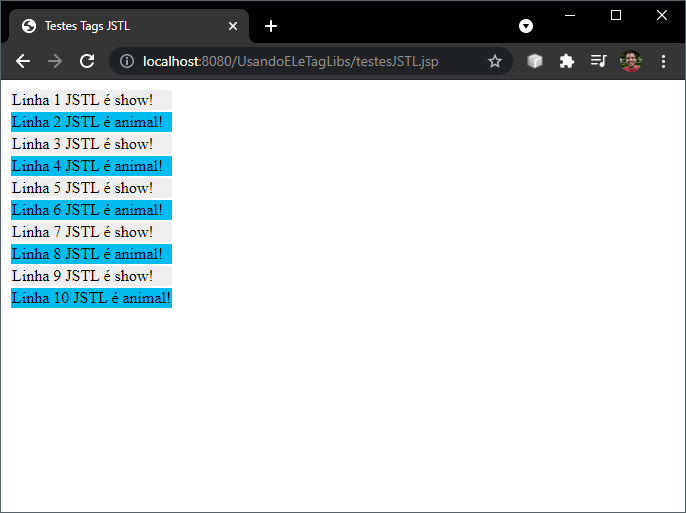
\includegraphics[scale=0.7]{imagens/cap03VisualizacaoTestesJSTL}
    \\\textbf{Fonte:} Elaborada pelo autor
    \label{fig:cap03VisualizacaoTestesJSTL}
\end{figure}
\FloatBarrier

Vamos analisar o código da Listagem~\thechapter.\ref{listagem:projetos/capitulo03/UsandoELeTagLibs/web/testesJSTL.jsp}. Talvez você tenha se assustado, mas não se preocupe, estou aqui para te explicar. Vamos começar pela primeira linha. Nessa linha, como em todos os JSPs que criamos até agora, usamos a diretiva \texttt{page}. As diretivas nos JSPs são delimitadas por \texttt{<\%@} e \texttt{\%>} e são usadas para realizar algumas configurações no Servlet que será gerado a partir do JSPs. A diretiva \texttt{page}, no nosso caso, é usada para configurar o \texttt{response} do Servlet, informando que ele vai conter um documento do tipo ``text/html'' (atributo \texttt{contentType}) e que o encoding utilizado (como os caracteres são codificados) é o UTF-8 (atributo \texttt{pageEncoding}). Veja que isso é análogo ao que estamos fazendo manualmente na primeira linha do método \inlineJavaCode{processRequest(...)} dos nossos Servlets.

Na linha 2 utilizamos a diretiva \texttt{taglib}. Essa diretiva vai permitir que nós digamos qual TagLib queremos utilizar. O atributo \texttt{uri} é usado para informarmos qual biblioteca de \textit{tags} queremos utilizar. No nosso caso, queremos utilizar as funcionalidades principais da JSTL, que são chamadas de ``core''. A \textit{Uniform Resource Identifier} (URI) para definir isso é a \texttt{http://java.sun.com/jsp/jstl/core}. O outro atributo, \texttt{prefix} (prefixo), nos permite definir um prefixo para usar as \textit{tags}. O prefixo padrão para a parte ``core'' da JSTL é ``c'', mas podemos usar o prefixo que quisermos. Para manter o padrão, iremos usar o ``c'' mesmo. Assim, quando qualquer desenvolvedor Web que conheça a JSTL bater o olho no código e ver alguma \textit{tag} que inicie com ``\texttt{c:}'' vai saber que a \textit{tag} que está sendo utilizada faz parte do core da JSTL.

Entre as linhas 12 e 20 definimos duas classes CSS. Sendo que uma usaremos para colorir o fundo das linhas pares de uma tabela, enquanto a outra será usada para colorir o fundo das linhas ímpares. A propriedade usada em ambas as classes é a \texttt{background} (fundo), sendo que em cada uma usamos uma cor diferente usando a notação \textit{Red Green Blue} (RGB) em hexadecimal. Nas linhas 25 e 40 delimitamos uma tabela.

\begin{saibaMais}
    Nunca ouviu falar de cores na notação em hexadecimal? De uma olhada nesses links: \url{http://dematte.at/colorPicker/}, \url{http://paletton.com/}, \url{https://pt.wikipedia.org/wiki/Tripleto_hexadecimal} e \url{http://en.wikipedia.org/wiki/Web_colors}
\end{saibaMais}

Na linha 26, usamos a \textit{tag} \inlineHTMLCode{<c:forEach>} (olhe o prefixo!), usada para iterar um determinado número de vezes ou sobre alguma lista de objetos. No nosso caso, queremos que o que está entre \inlineHTMLCode{<c:forEach>} e \inlineHTMLCode{</c:forEach>} seja executado dez vezes, pois definimos que a iteração deve iniciar em 1, usando o atributo \texttt{begin}, e ir até 10, usando o atributo \texttt{end}. Queremos também que o \textit{status} da iteração seja armazenado na variável \texttt{i}, definida no atributo \texttt{varStatus}. Então temos um \inlineJavaCode{for} que vai executar dez vezes. Durante estas dez iterações, vamos construir nossa tabela, inserindo linhas nela com apenas uma coluna, mas queremos que as linhas pares sejam coloridas usando a classe \inlineCSSCode{.linhaPar}, enquanto que as linhas ímpares sejam coloridas usando a classe \inlineCSSCode{.linhaImpar}. Sabemos que todo número par tem resto igual à zero numa divisão por dois, correto? Então precisamos saber em qual iteração estamos, calcular o resto e verificar se é zero. Se for, cria uma linha da tabela usando a classe \inlineCSSCode{.linhaPar}, caso contrário, usa \inlineCSSCode{.linhaImpar}.

Para criar séries de testes lógicos como numa estrutura \texttt{if/else}, nós usamos a \textit{tag} \inlineHTMLCode{<c:choose>} (\textit{to choose} = escolher) e dentro dela colocamos as condições que queremos testar usando a \textit{tag} \inlineHTMLCode{<c:when>} que é equivalente aos \texttt{if’s} e \texttt{else if’s} e, por fim, se necessário, usamos a \textit{tag} \inlineHTMLCode{<c:otherwise>} que é equivalente ao \inlineJavaCode{else}. Vamos analisar o código então: entre as linhas 27 e 38 nós definimos nossa estrutura condicional usando a \textit{tag} \inlineHTMLCode{<c:choose>}. Dentro dela, definimos na linha 28 uma \textit{tag} \inlineHTMLCode{<c:when>}, que testa (atributo \texttt{test}) se a divisão da propriedade \texttt{count} da variável \texttt{i} por dois é igual a zero (par). Note o uso da EL e que podemos executar operações aritméticas dentro dela! Se o resultado for \inlineJavaCode{true}, o número é par e o conteúdo deste \inlineHTMLCode{<c:when>} é gerado, ou seja, uma linha da tabela usando a classe \inlineCSSCode{.linhaPar}. Caso contrário, como não temos mais nenhum \inlineHTMLCode{<c:when>}, é gerado o código dentro do \inlineHTMLCode{<c:otherwise>}, que por sua vez também gera uma linha da tabela, só que usando a classe \inlineCSSCode{.linhaImpar}. Fique à vontade para mudar o conteúdo gerado dentro de cada linha, bem como as classes.

Viu como não é tão complicado? Na verdade é bem simples e fácil de usar, mas precisamos praticar para ficarmos craques. Depois dessa introdução à EL e a JSTL, nós já estamos quase prontos para começarmos o nosso primeiro projeto Web de verdade, mas ainda temos que formalizar algumas coisas que serão vistas no próximo Capítulo~\ref{cap:padroesDeProjeto}. Novamente, não se esqueça de praticar o que fizemos até agora.  


\section{Resumo}

Neste Capítulo nós aprendemos a criar um formulário que teve seus dados tratados por um Servlet, que por sua vez redirecionou o fluxo da aplicação para outra página JSP, utilizada para mostrar os dados informados no formulário. Com isso, tivemos uma noção do que é a EL e como ela funciona. Depois aprendemos um pouco sobre as \textit{tags} padrão da especificação dos JSPs e, por fim, aprendemos utilizar a JSTL em nosso projeto, além de fazermos alguns testes. No Capítulo~\ref{cap:padroesDeProjeto} vamos dar uma paradinha com os JSPs e Servlets para podermos aprender como estruturar um projeto Web que trabalha com banco de dados. Tenho certeza que você vai gostar bastante.


\section{Exercícios}

\begin{exercicioSemArquivo}{}{}{}
    Explique, com suas palavras, qual a importância da EL.
\end{exercicioSemArquivo}

\begin{exercicioSemArquivo}{}{}{}
    Justifique porque é melhor usar a JSTL ou qualquer outra TagLib ao invés de usar código Java diretamente nas JSPs.
\end{exercicioSemArquivo}

\section{Projetos}

\begin{projetoSemArquivo}{}{}{}
    Modifique o Projeto~\ref{cap:processamentoFormularios}.1 do Capítulo~\ref{cap:processamentoFormularios} para executar da mesma forma que o projeto criado neste Capítulo, ou seja, o formulário deve submeter os dados para um Servlet, que por sua vez deve criar e enviar um objeto através do \texttt{request} para um JSP, que deve exibir ao usuário usando EL.
\end{projetoSemArquivo}

\begin{projetoSemArquivo}{}{}{}
    Modifique o Projeto~\ref{cap:processamentoFormularios}.2 do Capítulo~\ref{cap:processamentoFormularios} para executar da mesma forma que o projeto criado neste Capítulo, ou seja, o formulário deve submeter os dados para um Servlet, que por sua vez deve criar e enviar um objeto através do \texttt{request} para um JSP, que deve exibir ao usuário usando EL.
\end{projetoSemArquivo}

\begin{projetoSemArquivo}{}{}{}
    Você já sabe que uma JSP na verdade é um Servlet não é mesmo? Será então que podemos definir na \texttt{action} de um formulário o endereço de um arquivo JSP ao invés de um Servlet? Crie um novo projeto Java Web, chamado ``JSPTrataFormulario'', onde você deve ter um formulário no \texttt{index.html} que contenha dois campos: nome e idade. A action deste formulário deve apontar para um arquivo JSP chamado ``exibeDadosForm.jsp'' (sem as aspas). Nesse arquivo, você deve mostrar os dados recebidos do formulário do \texttt{index.html} usando EL. Dica: para acessar os parâmetros do \texttt{request} usando EL, usa-se \texttt{\$\{param.nomeDoParametro\}}. Por exemplo, o parâmetro idade é acessado usando \texttt{\$\{param.idade\}}.
\end{projetoSemArquivo}

\begin{projetoSemArquivo}{}{}{}
    Crie um novo projeto Java Web, com o nome de ``TabelaArbitraria'', onde no \texttt{index.html} você deve ter um formulário que pede ao usuário que seja digita a quantidade de linhas e de colunas que ele deseja que uma tabela seja gerada. Aponte a \texttt{action} deste formulário para outro arquivo JSP, chamado ``montadorTabela.jsp'', que obtém os dados enviados pelo formulário do \texttt{index.html} usando EL e usa dois \inlineHTMLCode{<c:forEach>} aninhados para construir a tabela de dimensões arbitrárias. Monte a tabela somente se o tamanho de linhas e de colunas for maior que zero. Se não for, exiba uma mensagem ao usuário. Dica: para testar se duas condições são verdadeiras, ou seja, se \texttt{param.colunas > 0} e \texttt{param.linhas > 0}, use o operador \texttt{and} (e) da EL, enquanto o operador ``maior que'' é o \texttt{gt} (\textit{greater than}). Ou seja, \texttt{test="\$\{(param.linhas gt 0) and (param.colunas gt 0)\}"}.
\end{projetoSemArquivo}